\documentclass[12pt, twoside]{article}
\usepackage{jmlda}
\usepackage[utf8]{inputenc}
\usepackage[english,russian]{babel}
\usepackage{amssymb,amsfonts,amsmath,mathtext}
\usepackage{amsthm}
\usepackage{subfig}
\usepackage{array}
\usepackage{theorem}

\usepackage[all]{xy} % xy package for diagrams
\usepackage{array}
\usepackage{multicol}% many columns in slide
\usepackage{hhline}%tables
\usepackage{graphicx}
\usepackage{float}%"Плавающие" картинки
\usepackage{wrapfig}%Обтекание фигур (таблиц, картинок и прочего)
\graphicspath{{figures/}}
\newcommand{\hdir}{.}
\setcounter{secnumdepth}{6}
\newtheorem{def1}{Определение}
\newtheorem{theorem1}{Теорема}
\pgfplotsset{compat=1.18}
\begin{document}

\title
    %[Шаблон статьи для публикации] % краткое название; не нужно, если полное название влезает в~колонтитул
    {Классификация траекторий динамических систем с помощью физически-информированных нейросетей}
\author
    %[И.\,О.~Автор] % список авторов (не более трех) для колонтитула; не нужен, если основной список влезает в колонтитул
    {А.\,А.~Терентьев$^1$, С. К. Панченко$^1$, В.В. Стрижов}  %основной список авторов, выводимый в оглавление
   %[И.\,О.~Автор$^1$, И.\,О.~Соавтор$^2$
   %[И.\,О.~Фамилия$^{1,2}$] % список авторов, выводимый в заголовок; не нужен, если он не отличается от основного
\email
    {terentev.aa@phystech.edu; panchenko.sk@phystech.edu}
%\thanks
    %{
     %Работа выполнена при
     %частичной
     %финансовой поддержке РФФИ, проекты \No\ \No 00-00-00000 и %00-00-00001.
     %}
\organization
    {$^1$ФПМИ, МФТИ}
\abstract
    { В работе решается задача классификации траекторий физических систем. Динамика систем, соответствующих траекториям, моделируется лагранжианом, который аппроксимируется с помощью Лагранжевых нейронных сетей. Показано, что для динамики физических систем, соответствующим различным движениям, выполняется гипотеза компактности функциональных классов лагранжианов. На датасете PAMAP2 проведён эксперимент, результат которого подтверждают, что параматризация с помощью Лагранжевых нейронных сетей является достаточно общей для описания физических систем, а параметры -- информативным признаковым описанием для задачи классификации.
	
\bigskip
\noindent
\textbf{Ключевые слова}: \emph {физическая система; лагранжиан; лагарнжева нейронная сеть; гипотеза компактности}
}


%данные поля заполняются редакцией журнала
%\doi{10.21469/22233792}
%\receivedRus{28.02.2023}
%\receivedEng{January 01, 2017}

\maketitle
%\linenumbers

\section{Введение}
Одним из способов описания физических систем является лагранжев формализм. Преимущество такого подхода является общность: динамика каждой физической системы исчерпывающим образом описывается лагранжианом, который можно записывать в любых координатах, являющихся параметрами для данной системы. Именно лагранжиан предлагается использовать для классификации траекторий системы.

Для того, чтобы использовать лагранжеву механику, необходимо выбрать обобщенные координаты, которые полностью бы описывали поведение системы, иметь знания о Лагранжиане системы, который определяется как разница между кинетической энергией (T)\ и потенциальной энергией (V) 

\[L\left(\mathbf{q},\ \dot{\mathbf{q}}\right) \ =\ T\left(\mathbf{q},\ \dot{\mathbf{q}}\right)\ -\ V\left(\mathbf{q},\ \dot{\mathbf{q}}\right)  \]

\noindent
и величине обобщенных сил системы в случае внешних воздействий.
Динамика системы в таком случае описывается системой уравнений Эйлера-Лагранжа: 

\[ \frac{\partial L}{\mathbf{q}}\ -\ \frac{d}{dt}\ \frac{\partial L}{\partial\dot{\mathbf{q}}}=Q_x=0.\]

\noindent
Лагранжиан восстанавливается с помощью Лагранжевых нейронных сетей. Априорные знания о физике системы
являются преимуществом данной модели по сравнению с классическими нейронными сетями \cite{Thesis} \cite{article}.

Для лагранжианов физических систем утверждается гипотеза компактности: лагранжианы, отвечающие различным движениям, лежат в различных компактных и отделимых подмножествах-классах пространства моделируемых функций. На основе этого делается вывод о том, что векторы параметров функций, соответствующих различным классам, также компактны и отделимы в общем пространстве параметров. 

Для проверки гипотезы был произведен вычислительный эксперпимент на датасете PAMAP2, который содержит траектории движений человека во время различных активностей.

\section{Постановка задачи классификации траекторий физических систем}

Задана выборка с метками из $n$ траекторий: 

    $$\{ \mathcal{D}_j, z_j\}_{j=1}^n,$$ 
    где:
    \begin{itemize}

        \item[] $\mathcal{D}_j = \{ \mathbf{x}_i^{(j)}, \mathbf{y}_i^{(j)} \}_{i=1}^{m_j}$ ~-- $j$-ая траектория,

        \item[] $\mathbf{x}_i^{(j)} = (\mathbf{q}_i^{(j)}, \mathbf{\dot{q}}_i^{(j)})$ ~--  $i$-ые координаты и скорости $j$-ой траектории, 

        \item[] $\mathbf{y}_i^{(j)} = \mathbf{\dot{x}}_i^{(j)} = (\mathbf{\dot{q}}_i^{(j)}, \mathbf{\ddot{q}}_i^{(j)})$ ~--  $i$-ые скорости и ускорения $j$-ой траектории, 

        \item[] $\mathbf{q}_i^{(j)} \in \mathbb{R}^r$ ~-- вектор обобщенных координат,

        \item[] $r$ ~-- количество координат,

        \item[] $m_j$ ~-- длина $j$-ой траектории,

        \item[] $z_j \in \overline{1, K}$ ~-- метка $j$-ой траектории.
        
    \end{itemize}
        
    \subsection{Лагранжева динамика}\label{subsec:lagdyn}
    

        Сведём задачу моделирования лагранжиана системы к задаче регрессии. Регрессионная модель для траектории $D_j$ выбирается из класса лагранжевых нейронных сетей и представляет собой композицию:

        $$g_j \colon (\mathbf{x} | \mathbf{w}) \to L, \quad \mathbf{x} \in \mathbb{R}^{2 \times r},\  L \in \mathbb{R},$$

        $$ \mathbf{\kappa}: L \to \mathbf{y}, \quad \mathbf{y} \in \mathbb{R}^{2 \times r},$$


        $$ \mathbf{f}_j = \mathbf{\kappa} \circ g_j,$$
        
        где: 
    
        \begin{itemize}

            \item[] $g_j$ -- параметрическая функция, аппроксимириующая лагранжиан системы,

            \item[] $\mathbf{x} \in \mathbb{R}^{2 \times r}$ --  элемент траектории ($r$ обобщенных координат и $r$ обобщенных скоростей),

            \item[] $\mathbf{w} \in \mathbb{W}$ ~-- параметры аппроксимирующей лагранжиан модели,

            \item[] $L \in \mathbb{R}$ -- значение восстановленного лагранжиана,

            \item[] $\mathbf{\kappa}$ -- функция, реализующая уравнения Эйлера-Лагранжа для нахождения значения обобщенных скоростей и ускорений $\mathbf{y}$,

            \item[] $\mathbf{y} \in \mathbb{R}^{2 \times r}$ -- целевой вектор в задаче восстановления лагранжиана ($r$ обобщенных скоростей и $r$ обобщенных ускорений)

            \item[] $\mathbf{f}_j$ -- финальная композиция $g_j$ и $\mathbf{\kappa}$, представляющая собой Лагранжеву нейронную сеть.
            
        
        \end{itemize}

\newpage

        Задача моделирования динамики системы представлена в виде задачи минимизации квадратичной ошибки: 

        

        $$\mathcal{L}(\textbf{w}) = \mathcal{L}(\mathbf{w} | \mathcal{D}_j) = \frac{1}{m_j}\sum_{i=1}^{m_j} \| \hat{\mathbf{y}}_i^{(j)} - \mathbf{y}_i^{(j)} \|_2^2,$$

        
    
        $$\textbf{w}_j^* = \argmin_{\mathbf{w} \in \mathbb{W}} \left( \mathcal{L}(\textbf{w}) \right),$$

        \noindent
        где $\hat{\mathbf{y}}_i^{(j)} = \mathbf{f}_j (\mathbf{x}_i^{(j)} | \mathbf{w}) = \mathbf{\kappa} \big( g_j (\mathbf{x}_i^{(j)} | \mathbf{w}) \big) \in \mathbb{R}^{2 \times r}$ ~-- предсказанная динамика движения физической системы на $j$-ой траектории.
    
    \subsection{Задачи классификации траекторий по лагранжианам}

        После решения задачи моделирования лагранжиана получаем задачу классификации:

        $$\{\textbf{w}^*_j, z_j\}_{j=1}^n,$$
        где $\textbf{w}^*_j$ ~-- коэффициенты аппроксимированного лагранжиана $j$-ой траектории.
    
        Для ее решения используются различные методы классификации, среди которых: логистическая регрессия, гауссовская классификация, случайный лес.

\section{Гипотеза о компактности}




Пусть $\mathbb{L}$ -- функциональное линейное пространство лагранжианов всевозможных систем:

$$g: \mathbf{x} \to L, \quad g \in \mathbb{L},$$ 

\noindent
где $\mathbf{x} \in \mathbb{R}^{2 \times r}$ -- вектор обобщенных координат и скоростей, $L \in \mathbb{R}$ -- значение лагранжиана системы. Пусть также имеется  параметрическое семейство функций, аппроксимирующих лагранжиан, описанное в разделе 2.1,

$$\mathbb{L}_{\epsilon} = \{ g^{(\epsilon)} \colon (\mathbf{x} | \mathbf{w}) \to L \ | \ \mathbf{x} \in \mathbb{R}^{2 \times r}, \  L \in \mathbb{R},  
   \  \mathbf{w} \in \mathbb{W} \}, \quad \mathbb{L}_{\epsilon} \subset \mathbb{L},$$

\noindent
где $\mathbf{w}$ -- параметры функции из линейного пространства всевозможных значений параметров $\mathbb{W}$. Данное множество функций $\mathbb{L}_{\epsilon}$ представляет собой $\epsilon$-сеть в $\mathbb{L}$ при достаточной сложности модели в силу аппроксимационный свойств нейросетей.

Пусть каждой из $j = \overline{1, n}$ траекторий $\mathcal{D}_j$, соответствующих различным динамическим системам, описывающимся истинными Лагранжианами $g_j \in \mathbb{L}$ и принадлежащих различным классам $\mathcal{K}_{z_j}$, где $z_j \in \overline{1, K}$, сопоставлена аппроксимация лагранжиана $g_j^{(\epsilon)}(\mathbf{x}|\mathbf{w}_j^*) \in \mathbb{L}_{\epsilon}$ с помощью алгоритма, описанного в разделе 2.1. 
\newline

Основа классификации траекторий физических систем лежит в следующей гипотезе:

\begin{def1} 

По определению будем считать, что для пространства $\mathbb{L}$ с борлевской мерой выполняется гипотеза компактности с точностью $\delta$, если
В пространстве $\mathbb{L}$ мера пересечения различных классов мала
\[\delta\ >\ 0,\ \forall i,\ j,\ i\neq j\ \mu({K}_{z_i}\cap {K}_{z_j})\ <\ \delta\]
\end{def1}
Мы считаем, что рассматриваемое пространство $\mathbb{L}$ лежит в $L_2$ и соответсвенно везде далее считается $\mu$ - это борелевская мера на сепарбельном гильбертовом пространстве $L_2$. \cite{funcan} Данное пространство явлется сепарабельным, т.к. на нем можно ввест ортонормированный базис. 
Следующая же теорема позволит связать это с классификацией по параметрам нейронных сетей.
\begin{theorem1}
Пусть выполнятся для $\mathbb{L}$ гипотеза компактности с точностью $\delta$. А таже ${K}_{z_i}$ или их дополнения по мере ограничены $R$. Тогда также в пространстве $\mathbb{L}_{\epsilon}$ при $\epsilon$ стремящемся к нулю мера пересечения различных образов классов под действием $g_j^{\epsilon}$ мала

\[\delta\ >\ 0,\ \forall i,\ j,\ i\neq j\ \mu(g_j^{\epsilon}({K}_{z_i})\cap g_j^{\epsilon}({K}_{z_j})\ <\ 2\ *\delta\]

\end{theorem1}

\begin{proof}
 $\mu(z_i\cap z_j)\ <\ \mu(z_i\cap z_j) + \epsilon * R < 2\ *\ \delta $
\end{proof}


Если для системы $\mathbb{S}$ выполняется гипотеза компктности с точностью $\delta \ll min(\mu(z_{i}))$, то она поддается классификации.

\section{Лагранжевы нейронные сети}
%%%%%%%%%%%%%%%%%%%%%%%%%%%%%%%%%%%%%%%%%%%%%%%%%%%%%%%%%%%%%%%%%%%%%%%%%%

 
\paragraph{Уравнения Эйлера-Лагранжа}
Лагранжев формализм моделирует физическую систему с координатами $x_t = (q, \dot{q})$, которая начинается в состоянии $x_0$ и заканчивается в другом состоянии $x_1$. Определяется функционал, который называется действием
$$S=\int_{t_{0}}^{t_{1}} L d t,$$
 где $L$ -- лагранжиан системы. Действие определяет путь, по которому координаты $x_t$ пройдут из $x_0$ в $x_1$ в промежуток времени от $t_0$ до $t_1$. Путь минимизирует действие $S$, т.е. $\delta S = 0$. Это приводит к уравнению Эйлера-Лагранжа, определяющему динамику системы
$$\frac{d}{d t} \frac{\partial L}{\partial \dot{\mathbf{q}}}=\frac{\partial L}{\partial \mathbf{q}}$$

Ускорение каждой компоненты системы $ \ddot{\mathbf{q}}$ может быть напрямую получено из данного уравнения:

$$\begin{aligned} 
\frac{\partial}{\partial \dot{\mathbf{q}}} \frac{d L}{d t} 
&=\frac{\partial L}{\partial \mathbf{q}} \\ \frac{\partial}{\partial \dot{\mathbf{q}}}\left(\frac{\partial L}{\partial \mathbf{q}} \frac{d q}{d t}+\frac{\partial L}{\partial \dot{\mathbf{q}}} \frac{d \dot{\mathbf{q}}}{d t}\right) 
&=\frac{\partial L}{\partial \mathbf{q}} \\ \frac{\partial}{\partial \dot{\mathbf{q}}}\left(\frac{\partial L}{\partial \mathbf{q}} \dot{\mathbf{q}}+\frac{\partial L}{\partial \dot{\mathbf{q}}} \ddot{\mathbf{q}}\right) 
&=\frac{\partial L}{\partial \mathbf{q}} \\ \frac{\partial}{\partial \dot{\mathbf{q}}} \frac{\partial L}{\partial \mathbf{q}} \dot{\mathbf{q}}+\frac{\partial}{\partial \dot{\mathbf{q}}} \frac{\partial L}{\partial \dot{\mathbf{q}}} \ddot{\mathbf{q}} 
&=\frac{\partial L}{\partial \mathbf{q}} \\ \frac{\partial}{\partial \dot{\mathbf{q}}} \frac{\partial L}{\partial \dot{\mathbf{q}}} \ddot{\mathbf{q}} 
&=\frac{\partial L}{\partial \mathbf{q}}-\frac{\partial}{\partial \dot{\mathbf{q}}} \frac{\partial L}{\partial \mathbf{q}} \dot{\mathbf{q}} \\ \ddot{\mathbf{q}} 
&=\left(\frac{\partial}{\partial \dot{\mathbf{q}}} \frac{\partial L}{\partial \dot{\mathbf{q}}}\right)^{-1}\left[\frac{\partial L}{\partial \mathbf{q}}-\frac{\partial}{\partial \dot{\mathbf{q}}} \frac{\partial L}{\partial \mathbf{q}} \dot{\mathbf{q}}\right] \\ \ddot{\mathbf{q}} 
&=\left(\nabla_{\dot{\mathbf{q}} \dot{\mathbf{q}}} L\right)^{-1}\left[\nabla_{q} L-\left(\nabla_{\dot{\mathbf{q}}\mathbf{q}} L\right) \dot{\mathbf{q}}\right],
\end{aligned}$$

где гессиан $\left(\nabla_{\dot{\mathbf{q}\mathbf{q}}} L\right)_{i j}=\frac{\partial^{2} L}{\partial q_{j} \partial \dot{q}_{i}}$.

Таким образом, алгоритм моделирования динамики системы в лагранжевой динамике:
\begin{enumerate}
	\item Найти аналитические выражения для кинетической $(T)$ и потенциальной энергии $(V)$
	\item Получить лагранжиан $\mathcal{L} = T - V $
	\item Применить ограничение Эйлера-Лагранжа $\frac{d}{d t} \frac{\partial L}{\partial \mathbf{\dot{q}}} =\frac{\partial L}{\partial \mathbf{q}} $
	\item Решить получившуюся систему дифференциальных уравнений
\end{enumerate}


\subsection{Базовая модель Лагранжевой нейронной сети}

[Схема нейронной сети]

В работе [2] предложено в нейронную сеть $$f: \mathbf{X} = (\mathbf{q}, \mathbf{\dot{q}}) \rightarrow \mathbf{Y}$$
 добавить априорные знания о физике системы, моделируя лагранжиан:
$$f: \mathbf{X} = (\mathbf{q}, \mathbf{\dot{q}}) \rightarrow \mathbf{L};$$

Ключевой идеей является параметризация нейронной сетью лагранжиана $L$, получение выражения ограничения Эйлера-Лагранжа и обратное распространение ошибки через полученные ограничения
$$\ddot{\mathbf{q}} =\left(\nabla_{\dot{\mathbf{q}} \dot{\mathbf{q}}} L\right)^{-1}\left[\nabla_{q} L-\left(\nabla_{\dot{\mathbf{q}}\mathbf{q}} L\right) \dot{\mathbf{q}}\right].$$ 

В качестве нейронной сети берется полносвязная сеть с тремя слоями. Таким образом, для заданных координат  $(\mathbf{q}, \mathbf{\dot{q}})$ имеем модель с априорными знанями о законе сохранения энергии, с помощью которой можем получить динамику параметров $(\mathbf{\dot{q}}, \mathbf{\ddot{q}})$.



\section{Вычислительный эксперимент}
\paragraph{Цель эксперимента}
 \begin{enumerate}
        \item Проверить способность Лагранжевой нейросети моделировать физические системы достаточно эффективно по времени.
        \item Проверить правильность гипотензы о компактности и используя ее классифицировать траектории физические системы.
        \item Подобрать подходящий под данное распределения алгоритм классификации.
\end{enumerate}



\paragraph{Набор данных для базового эксперимета}
Набор данных с акселерометров из датасета PAMAP2.
\begin{itemize}
        \item Количество акселерометров: T = 3.
        \begin{itemize}
            \item Закрепленный на запастье преобладающей руки;
            \item Закрепленный на груди;
            \item Закрепленный на локте преобладающей руки.
        \end{itemize}
        \item Количество классов: K = 24.
        \item Количество испытуемых: M = 9.
        \item Каждая активность длилась минимум 1 час, частота сбора данных 100 Гц.
    \end{itemize}

\paragraph{Подготовка данных}
Для данных, полученных с аксселерометров, существует несколько проблем:
\begin{enumerate}
        \item Пропуски во временных рядаx.
        \item Временные ряды состоят только из линейных ускорений, либо угловых скоростей.
\end{enumerate}

Поэтому требуется восстановить пропущенные данные, иcпользуя интерполяцию, численное диффенцирование и интегрирование.

\begin{itemize}
        \item Датчики иногда могут пропускать один или два такта. Для востановления ряда используется сплайн-интерполяция, которая позволяет получить квадратичную точность от размеров сетки.
        \item Для восстановления ускорения, скорости и координат применяется численное дифференцированиe и интегрированиe.
\end{itemize}

Для дифференцирования используется центральная разность [формулу исправить лол тут бред немного]:
\[f'(x)\ =\ \frac{f(x_{k+1})\ -\ f(x_{k-1})}{2h}\]
\[\left|E(f)\right|\ \le \frac{h^2}{6}f^{(3)}\]
Для интегрирования используется Формула Кортеса:
    \[\int_{a}^{b}{f(x)dx}\approx\frac{h}{3}\sum_{k\ =\ 1}^{N\ -\ 1}{\Big(f(x_{k-1})+4f(x_k)+f(x_{k+1})\Big)}\],  
    \[\left|E(f)\right|\ \le\ \frac{(b-a)}{2880}h^4max\left|f^{(4)}\left(x\right)\right|\]


\paragraph{Эксперимент}
Берется подвыборка из датасета PAMAP2. Для каждого объекта применяется Лагранжева нейросеть, и с её помощью параметризуется лагранжиан.

Для проверки гипотезы построены 2D на Рисунке \ref{fig: 2D} и 3D на Рисунке \ref{fig: 3D}  графики для соответстенно двух и трех параметров, полученных понижением размерности методом главных компонент.


\begin{figure}[H]
    \centering
    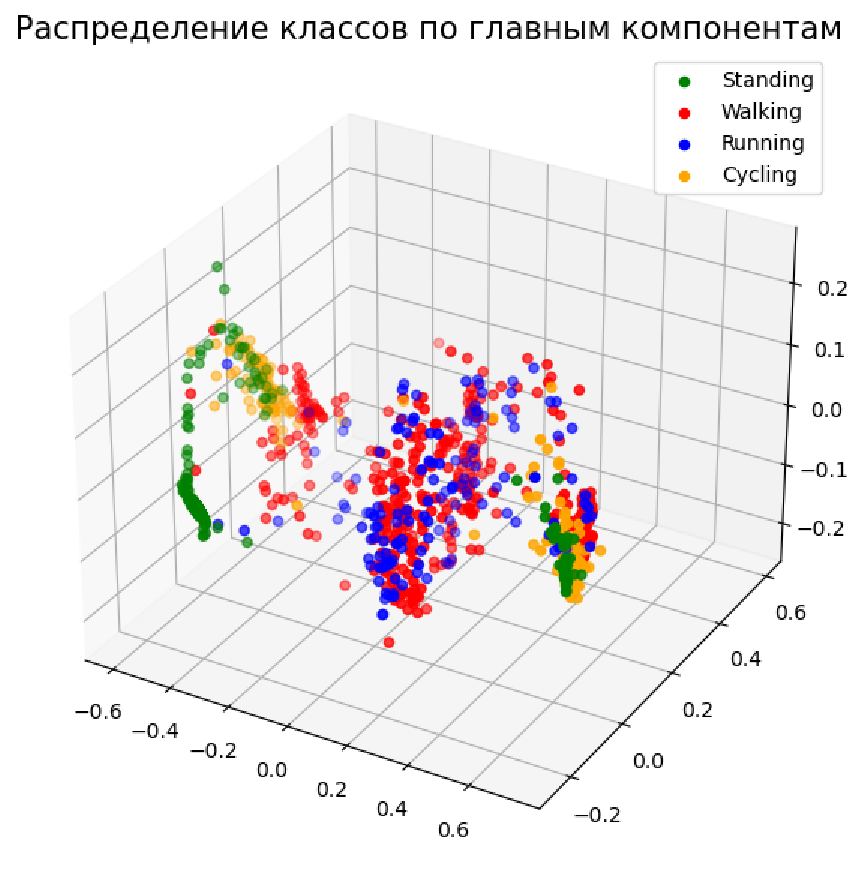
\includegraphics[scale = 0.8]{Parametrized_3D_class.pdf}
    \caption{Распределения данных в 3D}
    \label{fig: 3D}
\end{figure}

\begin{figure}[H]
    \centering
    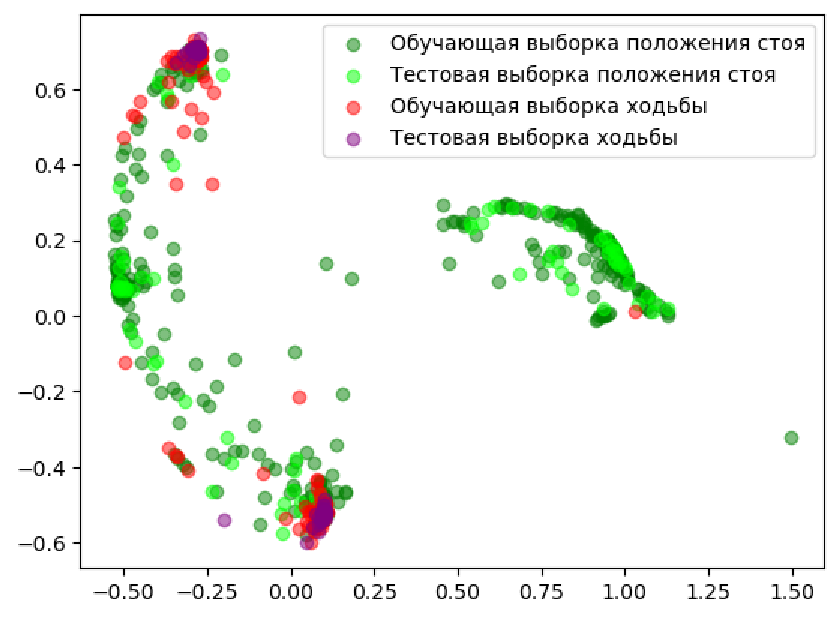
\includegraphics[scale = 0.8]{Parametrized_class_1.pdf}
    \caption{Распределения данных в 2D}
    \label{fig: 2D}
\end{figure}




%[ по возможности снабдить графики подробными подписями с описанием осей и сути происходящего на графике ]

На основе данных признаковых описаний, спроецированных на определенное число главных компонент, осуществляется классификация траекторий. На графике представлены значения точности, достигаемые тремя различными алгоритмами. Наилучший результат получился при использовании ядерного метода, при этом для классификации оказалось достаточно 10 главных компонент. Зависимость проиллюстрированна на Рисунке \ref{fig: PCA}.

\begin{figure}[H]
    \centering
    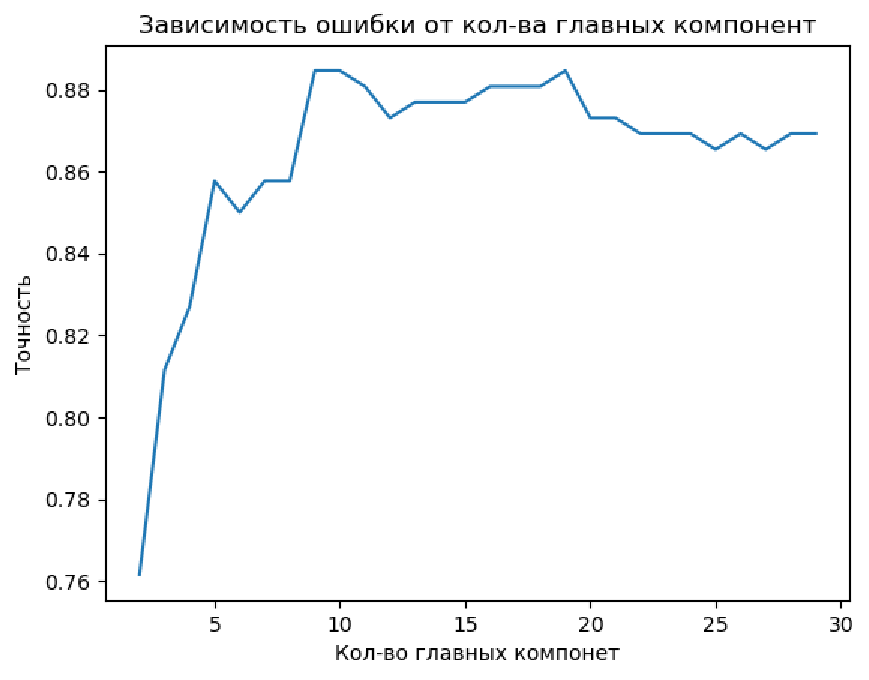
\includegraphics[scale = 0.8]{Error_per_PCA_1.pdf}
    \caption{Зависимость ошшибки от главных компонент}
    \label{fig: PCA}
\end{figure}

\begin{table}[h]
    \centering
    \begin{tabular}{|c|c|}
        \cline{1-2}
        Логистическая регрессия & $76\%$      \\ \hline
        Ядерный метод           & $88\%$      \\ \hline
        Случайный лес           & $84\%$      \\ \cline{1-2}                                
    \end{tabular}
    \caption{Зависимость ошшибки от выбранного метода}
    \label{tab: methodscomp}
\end{table}

\paragraph{Заключение}

Предложен метод классификации тракторий, не зависящий от физически не значимых изменений системы. Экспериментально показано, что классы траекторий отделимы в пространстве параметров Лагранжиана. Проведена классификация реальных траеторий движения частей тела людей при различных активностях. Подтверждена гипотеза компактности для рассматриваемых классов движений.


\begin{thebibliography}{99}

\bibitem{Thesis}
	\BibAuthor{Северилов~П.\,А.}
	Выбор оптимальной модели в задаче моделирования\\
        динамики физической системы~//
	URL: \BibUrl{https://github.com/severilov/master-thesis/blob/main/doc/Severilov2022MasterThesis_rus.pdf}.

\bibitem{article}
    \BibAuthor{M. Cranmer, S. Greydanus, S. Hoyer et al. }
    Lagrangian neural networks~//
    \BibJournal{ArXiv preprint.}, 2020.
	\BibDoi{Vol. abs/2003.04630}.
\bibitem{funcan}
    \BibAuthor{А.Г.Сергеев}
    Лекции по Функциональному анализу~//
    URL: \BibUrl{https://mi-ras.ru/noc/13_14/2/sergeev/funkan.pdf}.
\end{thebibliography}



%%%% если имеется doi цитируемого источника, необходимо его указать, см. пример в \bibitem{article}
%%%% DOI публикации, зарегистрированной в системе Crossref, можно получить по адресу http://www.crossref.org/guestquery/.


\end{document}
